\documentclass{book}
\usepackage[utf8x]{inputenc}
%\usepackage[french]{babel}

\usepackage{amssymb,amscd,latexsym,amsmath,amstext,amsfonts}
\usepackage{url}
\usepackage{xcolor}
\usepackage{multicol,float}
\usepackage{graphicx}
\usepackage{listings}

\lstdefinelanguage{Dedukti}
{
	inputencoding=utf8,
	extendedchars=true,
	numbers=none,
	numberstyle={},
	tabsize=2,
	basicstyle={\ttfamily\small\upshape},
	backgroundcolor=\color{lightgrey},
	keywords={abort,admit,apply,as,assert,assertnot,assume,compute,constant,definition,focus,in,injective,let,open,print,private,proof,proofterm,protected,qed,refine,reflexivity,require,rewrite,rule,set,simpl,symmetry,symbol,theorem,type,TYPE,why3,with, inductive},
	sensitive=true,
	keywordstyle=\color{blue},
	morecomment=[l]{//},
	commentstyle={\itshape\color{red}},
	string=[b]{"},
	stringstyle=\color{green},
	showstringspaces=false,
	literate={↪}{$\hookrightarrow$}1 {→}{$\rightarrow$}1 {Π}{$\Pi$}1
	{≔}{:=}1
	{⇒}{$\Rightarrow$}1
	{⊃}{$\Rightarrow$}1  %{$\supseq$}1
	{⇔}{$\Leftrightarrow$}1
	{∀}{$\forall$}1
	{∃}{$\exists$}1
	{⊥}{$\bot$}1
	{⊤}{$\top$}1
	{¬}{$\neg$}1
	{≡}{$\equiv$}1
	{ℕ}{$\mathbb{N}$}1
	{α}{$\alpha$}1 {π}{$\pi$}1 {τ}{$\tau$}1 {ω}{$\omega$}1 {λ}{$\lambda$}1
	{□}{$\square$}1 {⸬}{::}1
	{∧}{$\wedge$}1 {∨}{$\lor$}1
	{≤}{$\le$}1 {≠}{$\neq$}1 {∉}{$\notin$}1
	{×}{$\times$}1 {+}{+}1
	{⋅}{$\cdot$}1
}

\definecolor{beige}{rgb}{1.0, 0.99, 0.82}
\definecolor{orange_coq}{RGB}{255,69,0}
\definecolor{green_coq}{RGB}{0,100,0}
\definecolor{blue_coq}{RGB}{0,0,128}
\definecolor{blue_type}{RGB}{0,128,128}
\definecolor{brown_coq}{RGB}{88,41,0}
\definecolor{violet}{rgb}{0.54, 0.17, 0.89}


\lstdefinelanguage{Coq}
{
	inputencoding=utf8,
	extendedchars=true,
	numbers=none,
	numberstyle={}, %\tiny\color{black},
	tabsize=2,
	basicstyle=\small,
	sensitive=true,
	backgroundcolor=\color{beige},
	keywords={[0]Theorem, Lemma, Record, Inductive, Record, Fixpoint, Function, Definition, Axiom},
	keywordstyle={[0]\color{orange_coq} \bfseries},  
	keywords={[1]make, elt_list_member, member, elt_list_remove, remove, create, get_min, process_size, process_max, unsafe_create, sortWithoutDup},
	keywordstyle={[1]\color{blue}},
	keywords={[2]forall, if, then, else, match,with, end, let, in },
	keywordstyle={[2]\color{green_coq}},
	keywords={[4]Type, Prop}, 
	keywordstyle={[4]\color{blue_type}\bfseries},
	keywords={[5]Proof, Qed, Defined, Abort, 
		+, -, *, {, }}, 
	keywordstyle={[5]\color{violet} \bfseries},
	morecomment=[l]{(*},
	commentstyle={\itshape\color{brown_coq}\bfseries},
	string=[b]{"},
	stringstyle=\color{red},
	showstringspaces=false,
	literate={ -> }{$\rightarrow$}1 { <- }{$\leftarrow$}1 
	{<-> }{$\leftrightarrow$}1
	{\\/}{$\lor$}1 {/\\}{$\land$}1
	{~}{$\sim$}1
	{Π}{$\Pi$}1
	{≔}{$\coloneqq$}1
	{α}{$\alpha$}1 {π}{$\pi$}1 {τ}{$\tau$}1 {ω}{$\omega$}1
	{≤}{$\le$}1 {≠}{$\neq$}1 {∉}{$\notin$}1,
	% Pour le cadre du code
	aboveskip=1mm,
	%belowskip=-2mm,
	breakatwhitespace=false,
	breaklines=true,
	captionpos=b,
	escapeinside={\%*}{*)},
	extendedchars=true,  
	framexleftmargin=1pt,
	framextopmargin=3pt,
	framexbottommargin=6pt,
	frame=tb,
	keepspaces=true,
	% Code pas compris
	formfeed=newpage,
	morekeywords={models, lambda, forms}
	morekeywords={*,...},
	deletekeywords={...},
	rulecolor=\color{black},
	showspaces=false,
	showstringspaces=false,
	showtabs=false,
	stepnumber=1,
	%title=\lstname
}

\lstdefinelanguage{OCaml}
{
	inputencoding=utf8,
	extendedchars=true,
	numbers=none,
	numberstyle={},
	tabsize=2,
	basicstyle={\ttfamily\small\upshape},
	backgroundcolor=\color{yellow},
	keywords={let,rec,in,begin,end,match,with,fun,if,then,else,type,of},
	sensitive=true,
	keywordstyle=\color{green},
	commentstyle={\itshape\color{brown}},
	string=[b]{"},
	stringstyle=\color{red},
	showstringspaces=false
}


\lstdefinelanguage{K}
{
	inputencoding=utf8,
	extendedchars=true,
	numbers=none,
	numberstyle={},
	tabsize=2,
	basicstyle={\ttfamily\small\upshape},
	backgroundcolor=\color{green},
	keywords={module,imports,endmodule,syntax,configuration,context,rule},
	sensitive=true,
	keywordstyle=\color{blue},
	commentstyle={\itshape\color{brown}},
	string=[b]{"},
	stringstyle=\color{red},
	showstringspaces=false
}

\title{Un tour de monde de sémantique}
\author{Amélie Ledein}
\date{}

\newcommand{\Coqroot}{Coq_SemantiK}
\newcommand{\OCamlroot}{OCaml_SemantiK}
\newcommand{\Deduktiroot}{Dedukti_SemantiK}
\newcommand{\Kroot}{K_SemantiK}

\newcommand{\Introroot}{Book_SemantiK/0_Introduction}
\newcommand{\Arithroot}{Book_SemantiK/1_Expressions_Arith}
\newcommand{\Boolroot}{Book_SemantiK/2_Expressions_Bool}
\newcommand{\IMProot}{Book_SemantiK/3_IMP}
\newcommand{\MiniMLroot}{Book_SemantiK/4_MiniML}
\newcommand{\Objetroot}{Book_SemantiK/5_Objet}
\newcommand{\Concluroot}{Book_SemantiK/6_Conclusion}

\newcommand{\Texroot}{../..}

\begin{document}
	
	\maketitle
	
	%L'objectif de ce document est de présenter comme représenter des sémantiques dans différents langages existants, à savoir OCaml, Coq, Dedukti et $\mathbb{K}$. \\
	Pour ce faire, nous nous inspirons du cours de sémantique donné à l'ENSIIE, disponible dans le dossier PROG1\_lesson. Après avoir formaliser la syntaxe du langage à l'aide de la syntaxe BNF et de règles d'inférence, nous formaliserons la sémantique dénotationnelle ou opérationnelle sur ce langage. Ensuite, nous écrirons ces formalisations dans les 4 outils précédemment cités. Quand l'outil le permet, nous avons également réaliser des preuves de certaines propriétés sur ces sémantiques, comme le déterminisme ou l'équivalence entre sémantiques.
	
	Dans la suite de ce document, nous considérons que $n \in \mathbb{Z}$ et $x \in \mathbb{V}$ où $\mathbb{V}$ est un ensemble de variables.
	
	%
\chapter{Langage des expressions arithmétiques}

	\section{Syntaxe}

Nous pouvons formaliser la syntaxe de notre langage arithmétique grâce à la notation BNF : \\
$E_A$ ::= $n$ $|$ $x$ $|$ $E_A$ + $E_A$ $|$ $E_A$ - $E_A$ $|$ $E_A$ $\times$ $E_A$ $|$ $E_A$ / $E_A$ 
\vspace{1\baselineskip} \\
Un formalisme classiquement utilisé est d'écrire un système d'inférence : \\
\includegraphics[height=4cm]{\Arithroot/definition_inductive.png}
Cela revient à écrire un type inductif, ou une définition inductive. C'est ce que nous verrons lorsque nous écrirons cette syntaxe dans Coq ou dans Dedukti.

	\subsection{Traduction en OCaml}
	\lstinputlisting[language=OCaml, linerange={10-16}]{\OCamlroot/OCaml_exemple.ml}
	
	\subsection{Traduction en K}
	\lstinputlisting[language=K, linerange={1-11}]{\Kroot/K_exemple.k}

	\subsection{Traduction en Coq}
	\subsection{Traduction en Dedukti}


\section{Sémantique dénotationnelle}
Nous cherchons ici à interpréter des expressions arithmétiques, c'est-à-dire donner, à chaque expression arithmétique, une valeur appartenant à $\mathbb{V} = \mathbb{Z} \cup \{ Err \}$, où $Err$ dénote une erreur lors de l’interprétation.

\includegraphics[height=5cm]{\Arithroot/interpretation.png}

\includegraphics[height=5cm]{\Arithroot/schema_interpretation.png}

	\subsection{Traduction en OCaml}
Nous commençons d'abord par définir le type des valeurs possibles attendues ainsi que celui des valuations :
\lstinputlisting[language=OCaml, linerange={22-26}]{\OCamlroot/OCaml_exemple.ml}
Ensuite, nous définissons l'interprétation de chacun des opérateurs arithmétiques :
\lstinputlisting[language=OCaml, linerange={39-41,54-56,65-67,77-79}]{\OCamlroot/OCaml_exemple.ml}
Enfin, nous en déduisons l'évaluation de ces opérateurs :
\lstinputlisting[language=OCaml, linerange={91-97}]{\OCamlroot/OCaml_exemple.ml}

	\subsection{Traduction en K}
\lstinputlisting[language=K, linerange={13-39}]{\Kroot/K_exemple.k}

	\subsection{Traduction en Coq}
	\subsection{Traduction en Dedukti}

%\lstinputlisting[language=OCaml, linerange={137-142}]{\OCamlroot/OCaml_exemple.ml}

%\lstinputlisting[language=OCaml, linerange={157-173}]{\OCamlroot/OCaml_exemple.ml}

%\lstinputlisting[language=OCaml, linerange={220-225}]{\OCamlroot/OCaml_exemple.ml}
















\section{Sémantique opérationnelle d’évaluation à grands pas}

\includegraphics[height=5cm]{\Arithroot/eval_grands_pas.png}

Déterminisme \\
Proposition : \\
%∀a ∈ E A ∀σ ∈ V[Z] ∀v 1 , v 2 ∈ VA
%(ha, σi
%v 1 et ha, σi
%v 2 ) ⇒ v 1 = v 2
%Preuve : Par induction sur a.



Équivalence des sémantiques opérationnelle et
dénotationnelle

Propriétés Évaluation des expressions arithmétiques : variables

Expressions arithmétiques équivalentes (1) \\
Caractériser les expressions arithmétiques qui s’évaluent à la même valeur.
%a 1 ∼ a 2 ⇔ (∀v ∈ VA ∀σ ∈ V[Z] ha 1 , σi
%v ⇔ ha 2 , σi v)
%Proposition : $∼$ est une congruence. \\



\section{Sémantique opérationnelle d’évaluation à petits pas}

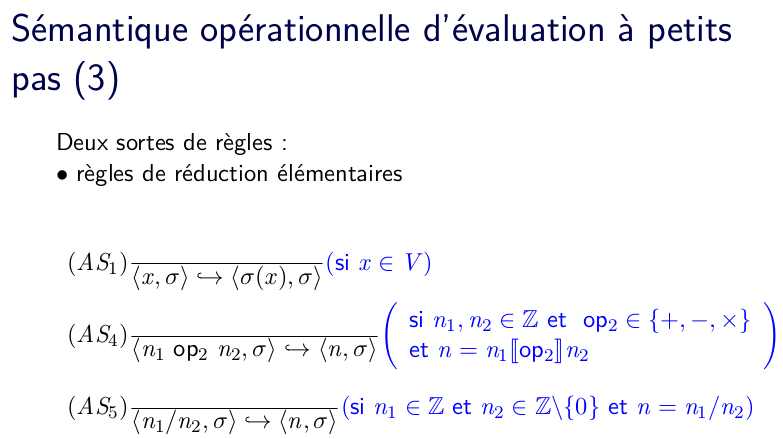
\includegraphics[height=5cm]{\Arithroot/eval_petits_pas_1.png}

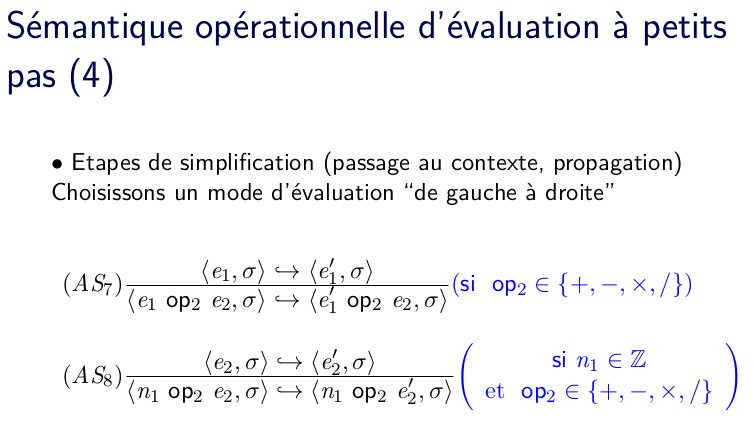
\includegraphics[height=5cm]{\Arithroot/eval_petits_pas_2.png}

déterministe


\section{Autre présentation : Contexte d'évaluation}

Cette autre présentation plus synthétique a été proposée par Andrew Wright et Matthias Felleisen.
Toutes les règles de simplification précédentes sont réduites à une seule : la règle de passage au contexte. \\

Cette présentation a été préférée lors de notre modélisation avec K :

\lstinputlisting[language=K, linerange={28-39}]{\Kroot/K_exemple.k}


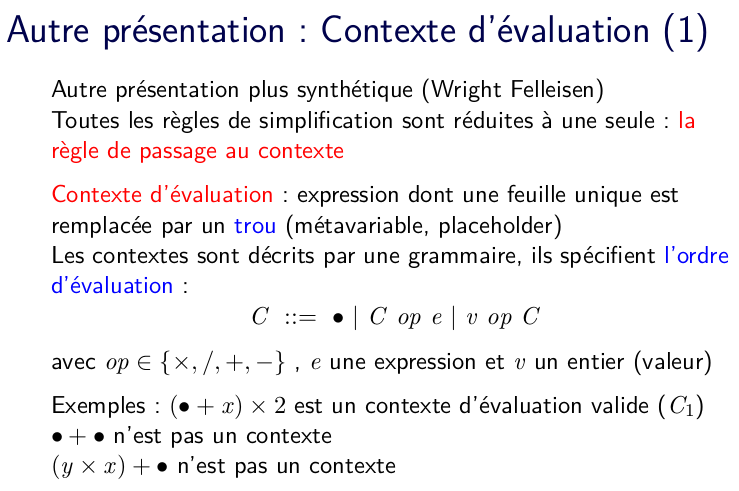
\includegraphics[height=5cm]{\Arithroot/contexte_eval_1.png}

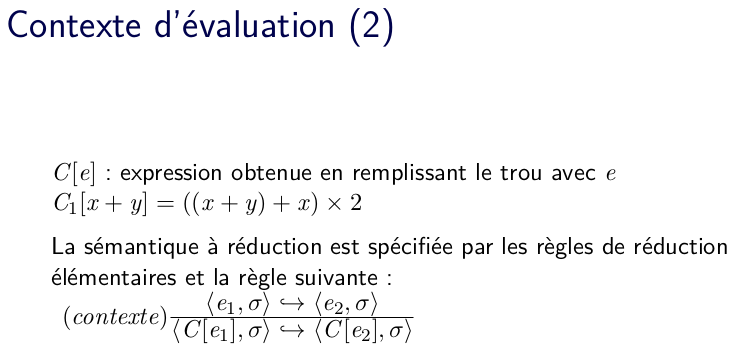
\includegraphics[height=5cm]{\Arithroot/contexte_eval_2.png}

Équivalence des sémantiques ?

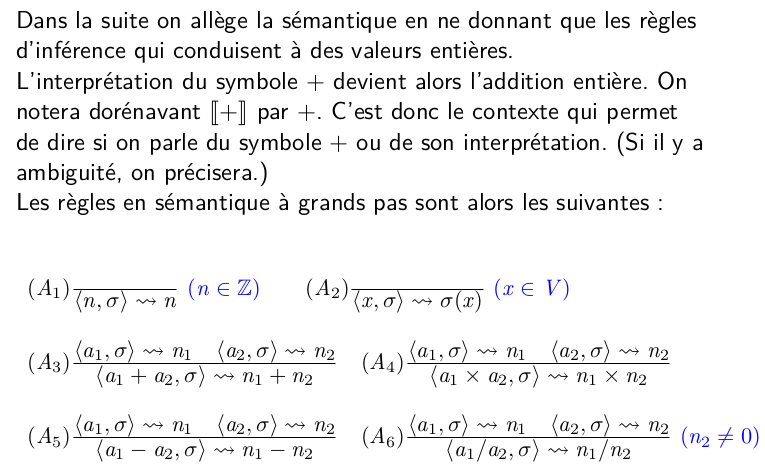
\includegraphics[height=5cm]{\Arithroot/simplification_notations.png}	
	
	%\chapter{Langage des expressions booléennes}

\section{Syntaxe}

Ce langage est une extension du langage des expressions arithmétiques qui nous venons de voir.
Nous pouvons également formaliser la syntaxe de notre langage booléen grâce à la notation BNF : \\
$E_B$ ::= true $|$ false $|$ $E_A$ $\le$ $E_A$ $|$ $E_A$ = $E_A$ $|$ not $E_B$ $|$ $E_B$ or $E_B$ $|$ $E_B$ and $E_B$
\vspace{1\baselineskip} \\
De même, nous obtenons le système d'inférence suivant : \\
\includegraphics[height=4cm]{\Boolroot/definition_inductive.png}

	\subsection{Traduction en OCaml}
	\lstinputlisting[language=OCaml, linerange={244-249}]{\OCamlroot/OCaml_exemple.ml}

	\subsection{Traduction en K}
	\lstinputlisting[language=K, linerange={41-51}]{\Kroot/K_exemple.k}

\section{Sémantique dénotationnelle}





\includegraphics[height=4cm]{\Boolroot/interpretation.png}

\includegraphics[height=4cm]{\Boolroot/schema_interpretation.png}

	\subsection{Traduction en OCaml}
	\lstinputlisting[language=OCaml, linerange={267-269,278-280,288-291,299-302,310-313}]{\OCamlroot/OCaml_exemple.ml}
	
	\lstinputlisting[language=OCaml, linerange={322-329}]{\OCamlroot/OCaml_exemple.ml}

	\subsection{Traduction en K}
	\lstinputlisting[language=K, linerange={53-84}]{\Kroot/K_exemple.k}


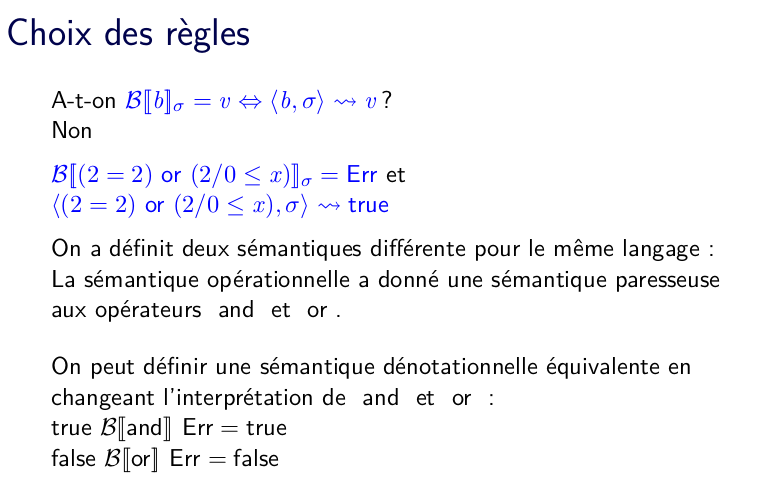
\includegraphics[height=4cm]{\Boolroot/choix_paresseux.png}










\section{Sémantique opérationnelle d’évaluation à grands pas}
Expressions booléennes équivalentes \\
$~$ est une congruence \\
Unicité d'un résultat

\includegraphics[height=4cm]{\Boolroot/eval_grands_pas.png}

\section{Sémantique opérationnelle d’évaluation à petits pas}
Exercice ?
	
	\subsection{Traduction en OCaml}

\lstinputlisting[language=OCaml, linerange={336-342}]{\OCamlroot/OCaml_exemple.ml}

\lstinputlisting[language=OCaml, linerange={353-362}]{\OCamlroot/OCaml_exemple.ml}

\lstinputlisting[language=OCaml, linerange={408-413}]{\OCamlroot/OCaml_exemple.ml}
	
	%
\chapter{Mini langage impératif : IMP}

\section{Syntaxe}

Ce langage est une extension du langage des expressions booléennes et arithmétiques qui nous venons de voir.
Nous pouvons également formaliser la syntaxe de notre mini langage impératif grâce à la notation BNF : \\
$E_C$ ::= skip $|$ $x$ := $E_A$ $|$ $E_C$ ; $E_C$ $|$ if $E_B$ then $E_C$ else $E_C$ $|$ while $E_B$ do $E_C$ \\
\vspace{1\baselineskip} \\
De même, nous obtenons le système d'inférence suivant : \\
\includegraphics[height=4cm]{\IMProot/definition_inductive.png} \\
A présent, nous allons pouvoir écrire des programmes impératifs !

	\subsection{Traduction en OCaml}
	\lstinputlisting[language=OCaml, linerange={454-456, 463-463, 502-508}]{\OCamlroot/OCaml_exemple.ml}

	\subsection{Traduction en K}
	\lstinputlisting[language=K, linerange={86-97}]{K_SemantiK/K_exemple.k}




\section{Sémantique opérationnelle d’évaluation à grands pas}

\includegraphics[height=4cm]{\IMProot/eval_grands_pas.png}


\section{Sémantique opérationnelle d’évaluation à petits pas}

	\subsection{Traduction en OCaml}

\lstinputlisting[language=OCaml, linerange={510-514}]{\OCamlroot/OCaml_exemple.ml}


\lstinputlisting[language=OCaml, linerange={526-537}]{\OCamlroot/OCaml_exemple.ml}

\lstinputlisting[language=OCaml, linerange={565-570}]{\OCamlroot/OCaml_exemple.ml}


\subsection{Traduction en K}
\lstinputlisting[language=K, linerange={99-124}]{K_SemantiK/K_exemple.k}
	
	%\chapter{MiniML}

		\section{Syntaxe}
Ce langage est indépendant des langages que nous venons de voir. Nous pouvons tout de même le formaliser grâce à la notation BNF : \\
$E_F$ ::= $n$ $|$ $x$ $|$ fun $x$ -$>$ $E_F$ $|$ $E_F$ $E_F$ $|$ $E_F$ + $E_F$
\vspace{1\baselineskip} \\
De même, nous obtenons le système d'inférence suivant : \\
\includegraphics[height=4cm]{\MiniMLroot/definition_inductive.png} \\
A présent, nous allons pouvoir écrire des programmes fonctionnels !

	\subsection{Traduction en OCaml}

\lstinputlisting[language=OCaml, linerange={602-608}]{\OCamlroot/OCaml_exemple.ml}

\lstinputlisting[language=OCaml, linerange={631-648}]{\OCamlroot/OCaml_exemple.ml}

\lstinputlisting[language=OCaml, linerange={659-675}]{\OCamlroot/OCaml_exemple.ml}

\lstinputlisting[language=OCaml, linerange={688-694}]{\OCamlroot/OCaml_exemple.ml}



\lstinputlisting[language=OCaml, linerange={726-739}]{\OCamlroot/OCaml_exemple.ml}

\lstinputlisting[language=OCaml, linerange={748-754}]{\OCamlroot/OCaml_exemple.ml}


\lstinputlisting[language=OCaml, linerange={778-784}]{\OCamlroot/OCaml_exemple.ml}

\lstinputlisting[language=OCaml, linerange={790-797}]{\OCamlroot/OCaml_exemple.ml}

\lstinputlisting[language=OCaml, linerange={808-827}]{\OCamlroot/OCaml_exemple.ml}

\lstinputlisting[language=OCaml, linerange={840-846}]{\OCamlroot/OCaml_exemple.ml}

\lstinputlisting[language=OCaml, linerange={881-896}]{\OCamlroot/OCaml_exemple.ml}

\lstinputlisting[language=OCaml, linerange={905-911}]{\OCamlroot/OCaml_exemple.ml}



	
		\section{Appel par valeur}
		
		\subsection{Sémantique opérationnelle d’évaluation à grands pas}

\includegraphics[height=4cm]{\MiniMLroot/Appel_par_valeur/eval_grands_pas.png}		
		
		\subsection{Sémantique opérationnelle d’évaluation à petits pas}
		
\includegraphics[height=4cm]{\MiniMLroot/Appel_par_valeur/eval_petits_pas.png}		
		
		\section{Appel par nom}
		
		\subsection{Sémantique opérationnelle d’évaluation à grands pas}

\includegraphics[height=4cm]{\MiniMLroot/Appel_par_nom/eval_grands_pas.png}		
		
		\subsection{Sémantique opérationnelle d’évaluation à petits pas}

\includegraphics[height=4cm]{\MiniMLroot/Appel_par_nom/eval_petits_pas.png}
	
	%
\chapter{Mini langage objet}

$e$ ::= $x$ $|$ $e$.$l$ $|$ [$l1$=$\zeta$($x1$)$e1$,...,$ln$=$\zeta$($xn$)$en$] $|$ $e$.$l$:=$\zeta$($x$)$e$ $|$ $n$ $|$ $e$+$e$

	
	%\input{\Concluroot/conclusion.tex}
	
\end{document}